% chktex-file 8
\section{Exercise 1} 

\subsection*{Part (a)}

On a base labyrinth we define a $N\times N$ grid where we enumerate each position with the lexicographical ordering. In particular, for the case $N = 7$ we have the following ordering,

\begin{figure}[H]
    \centering
    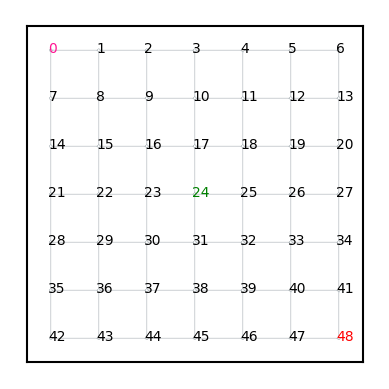
\includegraphics[width=0.6\textwidth]{../pictures/numbering.png}
\end{figure}

We put 2 exits on this graph, each one corresponds to an absorbing state. In the previous image, the absorbing states are $0$ (pink) and $48$ (red). Furthermore, unless we put a wall between to positions in the grid, each vertex on the position $k$ is connected (if possible) with $k+1$ (right), $k-1$ (left), $k+N$ (up), $k-N$ (down).

For the walls I made a graphical interface that lets the user interact with which walls the labyrinth should have. You can find the \href{https://colab.research.google.com/drive/1S1VUt5ehHkPthAicE4mKvIPgcmJihZ6H?usp=sharing}{\textcolor{blue}{\underline{program clicking here}}} The program lets the user:
\begin{itemize}
    \item Move the starting points and the exits.
    \item Change the size of the grid.
    \item See labels for the average time of absorption on each position.
    \item See the labels for the probability of absorption of \textcolor{magenta}{Exit 1} vs \textcolor{red}{Exit 2} on each position.
\end{itemize}

\begin{figure}[H]
    \begin{tabular}{cc}
      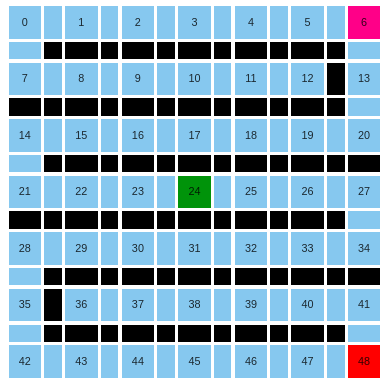
\includegraphics[width=70mm]{../pictures/interface.png} &   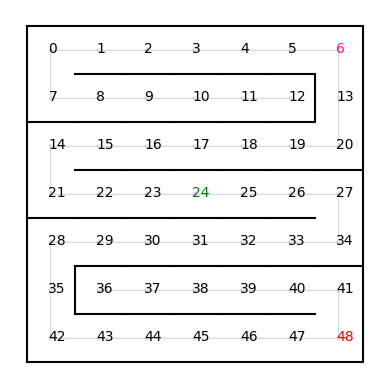
\includegraphics[width=70mm]{../pictures/216-1.png} \\
    Button Graphical Interface & Labyrinth (All Labels Off) \\[6pt]
     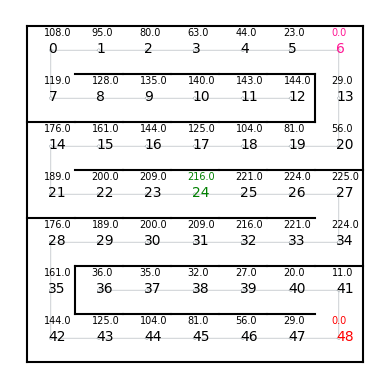
\includegraphics[width=70mm]{../pictures/216-2.png} &   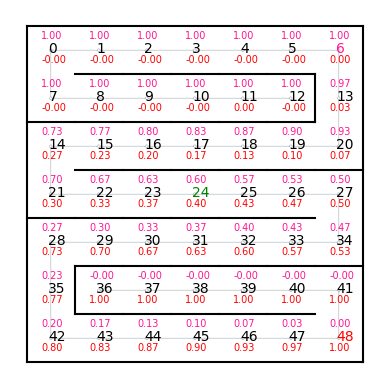
\includegraphics[width=70mm]{../pictures/216-3.png} \\
    Average Absorption Times Labels On & Absorption Probabilities Labels On \\[6pt]
    \end{tabular}
\end{figure}

\subsection*{Part (b)}

Let $A$ be the graph $N^2\times N^2$ matrix that describes all the allowed connections of the vertices in the labyrinth when there's no wall between them. In general,
\[ A_{k,l} = \begin{cases}
    1 & \mbox{if } l \in \{k+1,k-1,k+N, k-N\}\\
    0 & \mbox{otherwise (or when k and l are too far)}
\end{cases},\; k,l \in \{0,1,\ldots,N^2-1\} \]    
Let $W = \{(k,l) \in W\}$ be a set of walls in the labyrinth, which is a subset of all possible edges allowed by the graph $A_{k,l}$. Then, we define our labyrinth graph with the following matrix
\[ M_{k,l} = A_{k,l} - \1\{(k,l)\in W\},\]
which is the set of all the allowed edges that aren't obstructed by a wall. Let $m_k = \sum_{l = 0}^{N^2}M_{k,l}$ be the sum of the entries of $k$-th row in the matrix $M$, and let $k_1, k_2$ be the indices for the 2 exits, the transition matrix for our random walk on the graph is defined by
\[ \Pi_{k,l} = \frac{M_{k,l}}{m_k}, \; k,l \not\in \{k_1,k_2\}, \]
\[ \Pi_{k_1,k_1} = \Pi_{k_2,k_2} = 1,\hspace*{2em} \Pi_{k_1,l} = \Pi_{k_2,l} = 0,\; l\neq k_1,k_2\mbox{ (respectively)}. \]

Without the walls, the graph of the previous example would look like:
\begin{figure}[H]
    \centering
    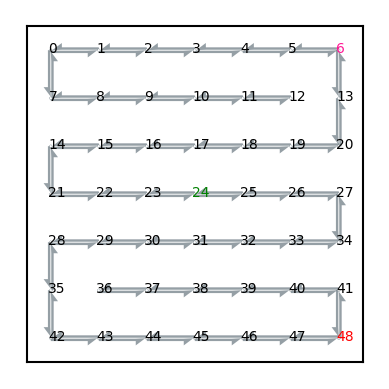
\includegraphics[width=0.6\textwidth]{../pictures/216-4.png}
\end{figure}

\subsection*{Part (c)}

Let $A = \{k_1,k_2\}$. For $l\in A$, the linear system for the vector $g_l = {(P\{Z_{T_A}\;|\; X_0 = k\})}_{k<N^2}$ is the following:
\[ \left\{\begin{array}{ccl}
    \sum_{k = 0}^{N^2} \Pi_{k,m} \cdot g_l(m) - g_l(k) & = 0, & \mbox{For }k \not\in A\\
    g_l(k) & = 0, & \mbox{For }k \in A,\; k\neq l\\
    g_l(l) & = 1
\end{array}\right. \]

Then, we can express this system as follows
\[ A \cdot g_l = b_l, \]
where, for $l\in A$, we define $b_l \in \R^{N^2}$ as 
\[ b_l(k) = \begin{cases}
    1 & k = l\\
    0 & k\neq l.
\end{cases} \]
If $I_k$ is the $k$-th row of the identity matrix and $\Pi_k$ the $k$-th row of $\Pi$, then the $k$-th row of $A$ is defined as
\[ A_{k} = \begin{cases}
    I_k & k\in A\\
    \Pi_{k}-I_k & k\not\in A
\end{cases}\]

Thus, the probability of going from \textcolor{Green}{Start 24} to \textcolor{magenta}{Exit 6} is 0.6 and \textcolor{red}{Exit 48} is 0.4. Note that all the other probabilities starting from other positions also sum 1.0.

\begin{figure}[H]
    \centering
    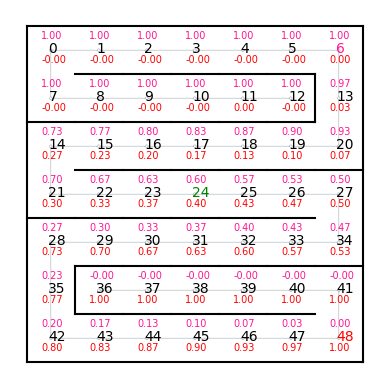
\includegraphics[width=0.6\textwidth]{../pictures/216-3.png}
\end{figure}

\subsection*{Part (d)}
For the average absorption time we have the following linear system
\[ \left\{\begin{array}{ccl}
    h_A(k) - \sum_{k = 0}^{N^2} \Pi_{k,l} \cdot h_A(l)  & = 1, & \mbox{For }k \not\in A\\
    h_A(k) & = 0, & \mbox{For }k \in A.\\
\end{array}\right. \]
Then, we can express this system as
\[ B\cdot h_A = b_A, \]
where, $b_A$ is defined as
\[ b_A(k) = \begin{cases}
    1 & k \not\in A\\
    0 & k\in A
\end{cases}, \]
and the rows of $B$ as
\[ B_k = \begin{cases}
    I_k - \Pi_k & k \not\in A\\
    I_k & k \in A.
\end{cases} \]

After solving the system for the previous example we obtain
\begin{figure}[H]
    \centering
    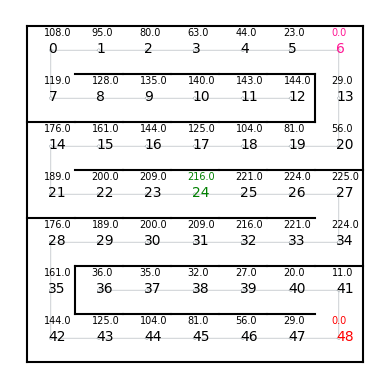
\includegraphics[width=0.6\textwidth]{../pictures/216-2.png}
\end{figure}

\subsection*{Part (e)}

If we keep the 2 exits at $\{6,48\}$ but we reflect the walls over both $x,y$ axis we obtain the following labyrinth:

\begin{figure}[H]
    \begin{tabular}{cc}
      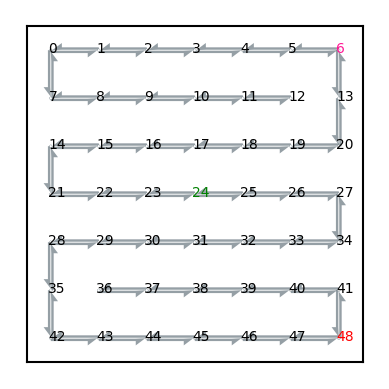
\includegraphics[width=70mm]{../pictures/216-4.png} &   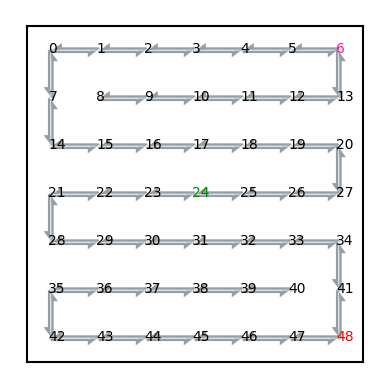
\includegraphics[width=70mm]{../pictures/inv-4.png} \\
    Original Graph & Reflected Graph \\[6pt]
    \end{tabular}
\end{figure}

Now, the absorption probabilities should be the following

\begin{figure}[H]
    \centering
    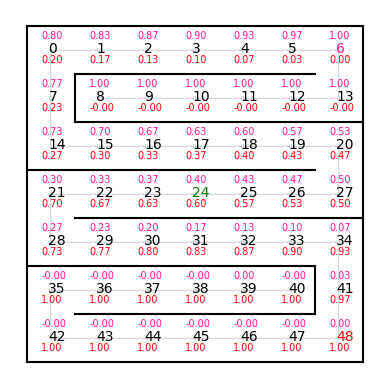
\includegraphics[width=0.6\textwidth]{../pictures/inv-3.png}
\end{figure}

Thus, according to the previous image, the probability of going from \textcolor{Green}{Start 24} to \textcolor{magenta}{Exit 6} is 0.4 and \textcolor{red}{Exit 48} is 0.6. Which is the oposite to the other labyrinth.

\subsection*{Part (f) - Double Time}

We remove from the original graph the edge $(6,13)$ and add the edge $(12,13)$. Then, the distance between \textcolor{Green}{Start 24} and \textcolor{magenta}{Exit 6} is doubled. For some reason, this also doubles the expected time to reach one of the exits. I believe that this is associated to the fact that every point connected to both exits has to pass through \textcolor{Green}{Start 24}, but I'm not sure.

\begin{figure}[H]
    \begin{tabular}{cc}
      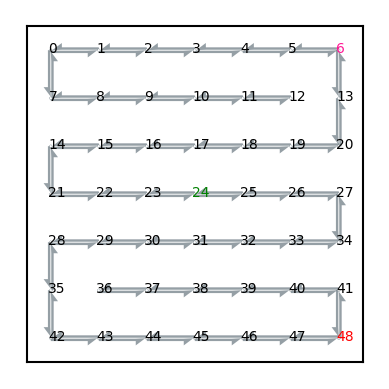
\includegraphics[width=70mm]{../pictures/216-4.png} &   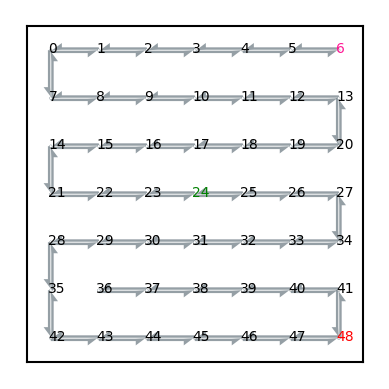
\includegraphics[width=70mm]{../pictures/432-4.png} \\
    Original Graph & Double Time Graph \\[6pt]
    \end{tabular}
\end{figure}

Now, this new graph takes in average double the time of the original time to reach one of the exits

\begin{figure}[H]
    \centering
    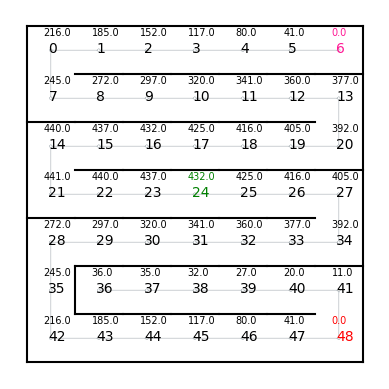
\includegraphics[width=0.6\textwidth]{../pictures/432-2.png}
\end{figure}

\subsection*{Part (f) - Half Time}

We removed the edges $\{(23,24),(16,17)\}$ and added the edges $\{(9,16),(17,24)\}$. With the same idea, this halved the distance between \textcolor{Green}{Start 24} and \textcolor{magenta}{Exit 6}.

\begin{figure}[H]
    \begin{tabular}{cc}
      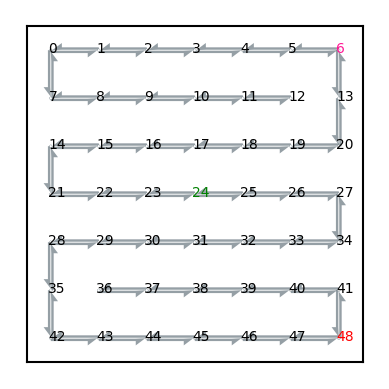
\includegraphics[width=70mm]{../pictures/216-4.png} &   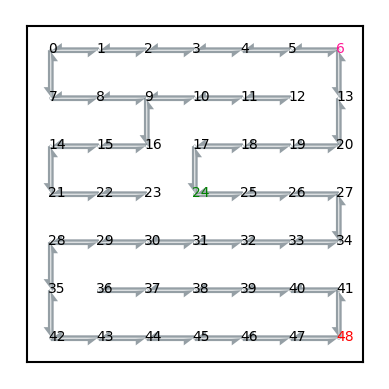
\includegraphics[width=70mm]{../pictures/108-4.png} \\
    Original Graph & Half Time Graph \\[6pt]
    \end{tabular}
\end{figure}

Now, this new graph takes in average half the time of the original to reach one of the exits

\begin{figure}[H]
    \centering
    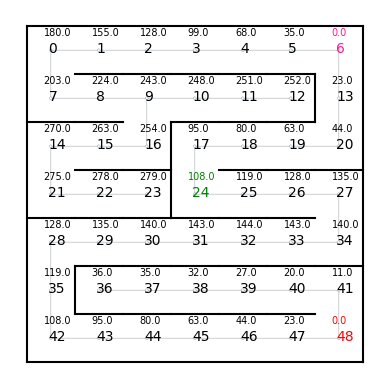
\includegraphics[width=0.6\textwidth]{../pictures/108-2.png}
\end{figure}
